\documentclass{standalone}
\usepackage{tikz}
\usetikzlibrary{patterns, positioning}


\begin{document}
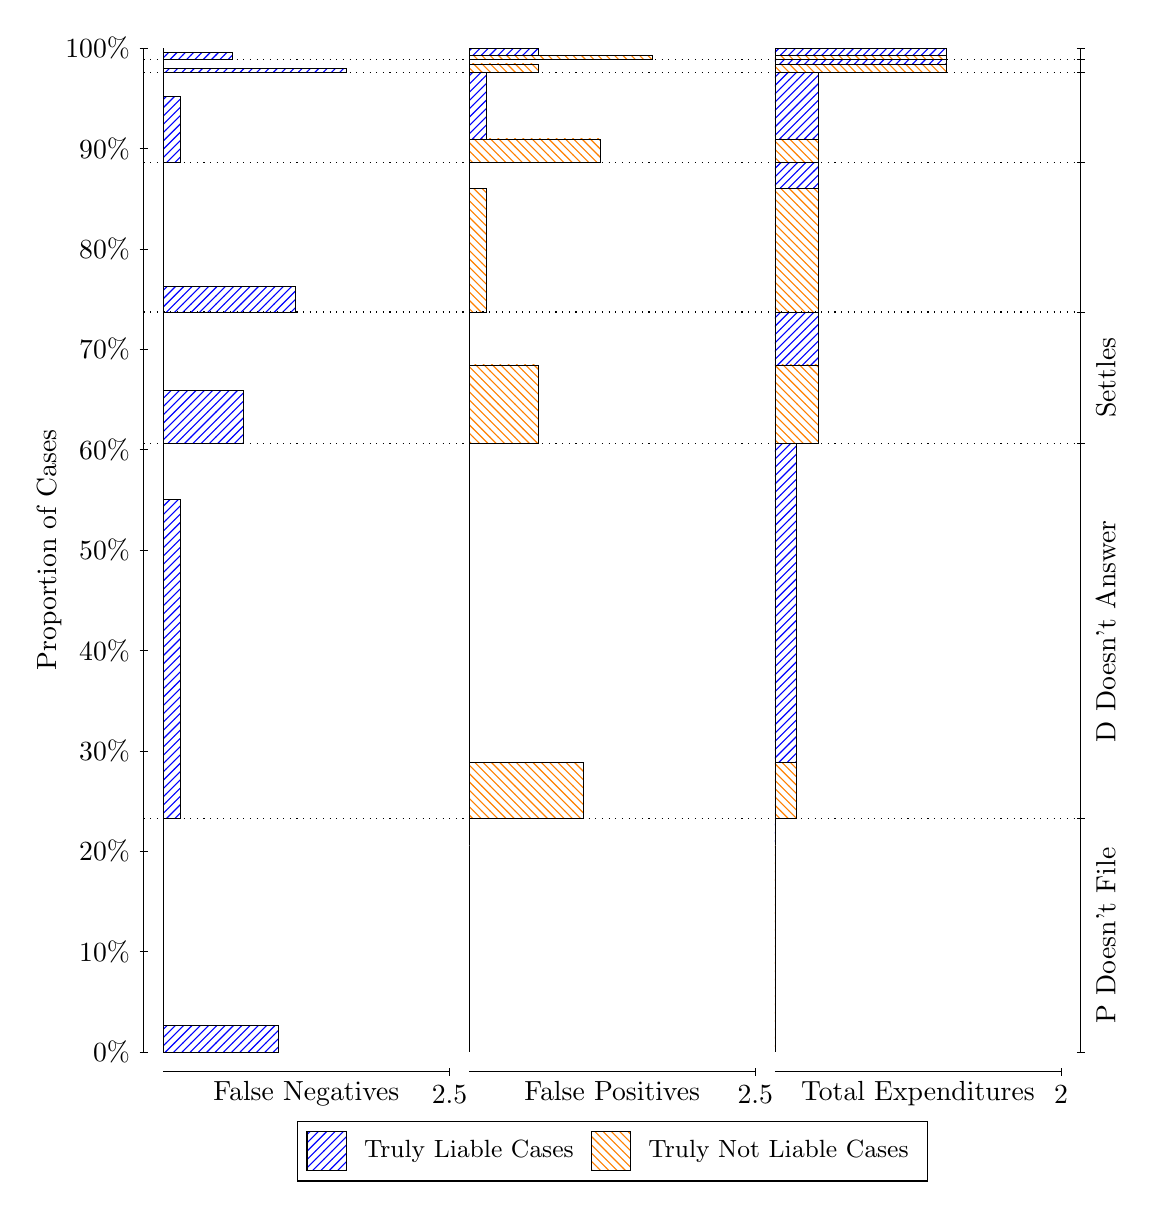
\begin{tikzpicture}
\draw[black, very thin] (1.5,1.75) -- (1.5,14.5);
\node[rotate=90, text=black, anchor=center] at (0.3, 8.125) {Proportion of Cases};
\draw[black, very thin] (1.45,1.75) -- (1.55,1.75);
\node[text=black, anchor=east] at (1.45, 1.75) {0\%};
\draw[black, very thin] (1.45,3.025) -- (1.55,3.025);
\node[text=black, anchor=east] at (1.45, 3.025) {10\%};
\draw[black, very thin] (1.45,4.3) -- (1.55,4.3);
\node[text=black, anchor=east] at (1.45, 4.3) {20\%};
\draw[black, very thin] (1.45,5.575) -- (1.55,5.575);
\node[text=black, anchor=east] at (1.45, 5.575) {30\%};
\draw[black, very thin] (1.45,6.85) -- (1.55,6.85);
\node[text=black, anchor=east] at (1.45, 6.85) {40\%};
\draw[black, very thin] (1.45,8.125) -- (1.55,8.125);
\node[text=black, anchor=east] at (1.45, 8.125) {50\%};
\draw[black, very thin] (1.45,9.4) -- (1.55,9.4);
\node[text=black, anchor=east] at (1.45, 9.4) {60\%};
\draw[black, very thin] (1.45,10.675) -- (1.55,10.675);
\node[text=black, anchor=east] at (1.45, 10.675) {70\%};
\draw[black, very thin] (1.45,11.95) -- (1.55,11.95);
\node[text=black, anchor=east] at (1.45, 11.95) {80\%};
\draw[black, very thin] (1.45,13.225) -- (1.55,13.225);
\node[text=black, anchor=east] at (1.45, 13.225) {90\%};
\draw[black, very thin] (1.45,14.5) -- (1.55,14.5);
\node[text=black, anchor=east] at (1.45, 14.5) {100\%};

\draw[black, very thin] (13.4,1.75) -- (13.4,14.5);
\draw[black, very thin] (13.35,1.75) -- (13.45,1.75);
\node[anchor=west] at (13.35, 1.75) {};
\draw[black, very thin] (13.35,4.7131) -- (13.45,4.7131);
\node[anchor=west] at (13.35, 4.7131) {};
\draw[black, very thin] (13.35,9.4768) -- (13.45,9.4768);
\node[anchor=west] at (13.35, 9.4768) {};
\draw[black, very thin] (13.35,11.147) -- (13.45,11.147);
\node[anchor=west] at (13.35, 11.147) {};
\draw[black, very thin] (13.35,13.046) -- (13.45,13.046);
\node[anchor=west] at (13.35, 13.046) {};
\draw[black, very thin] (13.35,14.187) -- (13.45,14.187);
\node[anchor=west] at (13.35, 14.187) {};
\draw[black, very thin] (13.35,14.354) -- (13.45,14.354);
\node[anchor=west] at (13.35, 14.354) {};
\draw[black, very thin] (13.35,14.5) -- (13.45,14.5);
\node[anchor=west] at (13.35, 14.5) {};

\draw[black, very thin, pattern color=blue, pattern=north east lines] (1.75,1.75) rectangle (3.2033,2.0916);
\draw[black, very thin, pattern color=orange, pattern=north west lines] (1.75,2.0916) rectangle (1.75,4.7131);
\draw[black, very thin, pattern color=blue, pattern=north east lines] (1.75,4.7131) rectangle (1.968,8.7631);
\draw[black, very thin, pattern color=orange, pattern=north west lines] (1.75,8.7631) rectangle (1.75,9.4768);
\draw[black, very thin, pattern color=blue, pattern=north east lines] (1.75,9.4768) rectangle (2.7673,10.149);
\draw[black, very thin, pattern color=orange, pattern=north west lines] (1.75,10.149) rectangle (1.75,11.147);
\draw[black, very thin, pattern color=blue, pattern=north east lines] (1.75,11.147) rectangle (3.4213,11.472);
\draw[black, very thin, pattern color=orange, pattern=north west lines] (1.75,11.472) rectangle (1.75,13.046);
\draw[black, very thin, pattern color=blue, pattern=north east lines] (1.75,13.046) rectangle (1.968,13.886);
\draw[black, very thin, pattern color=orange, pattern=north west lines] (1.75,13.886) rectangle (1.75,14.187);
\draw[black, very thin, pattern color=blue, pattern=north east lines] (1.75,14.187) rectangle (4.0753,14.242);
\draw[black, very thin, pattern color=orange, pattern=north west lines] (1.75,14.242) rectangle (1.75,14.354);
\draw[black, very thin, pattern color=blue, pattern=north east lines] (1.75,14.354) rectangle (2.622,14.445);
\draw[black, very thin, pattern color=orange, pattern=north west lines] (1.75,14.445) rectangle (1.75,14.5);
\draw[black, very thin, pattern color=orange, pattern=north west lines] (5.6333,1.75) rectangle (5.6333,4.3715);
\draw[black, very thin, pattern color=blue, pattern=north east lines] (5.6333,4.3715) rectangle (5.6333,4.7131);
\draw[black, very thin, pattern color=orange, pattern=north west lines] (5.6333,4.7131) rectangle (7.0867,5.4269);
\draw[black, very thin, pattern color=blue, pattern=north east lines] (5.6333,5.4269) rectangle (5.6333,9.4768);
\draw[black, very thin, pattern color=orange, pattern=north west lines] (5.6333,9.4768) rectangle (6.5053,10.475);
\draw[black, very thin, pattern color=blue, pattern=north east lines] (5.6333,10.475) rectangle (5.6333,11.147);
\draw[black, very thin, pattern color=orange, pattern=north west lines] (5.6333,11.147) rectangle (5.8513,12.721);
\draw[black, very thin, pattern color=blue, pattern=north east lines] (5.6333,12.721) rectangle (5.6333,13.046);
\draw[black, very thin, pattern color=orange, pattern=north west lines] (5.6333,13.046) rectangle (7.3047,13.347);
\draw[black, very thin, pattern color=blue, pattern=north east lines] (5.6333,13.347) rectangle (5.8513,14.187);
\draw[black, very thin, pattern color=orange, pattern=north west lines] (5.6333,14.187) rectangle (6.5053,14.299);
\draw[black, very thin, pattern color=blue, pattern=north east lines] (5.6333,14.299) rectangle (5.6333,14.354);
\draw[black, very thin, pattern color=orange, pattern=north west lines] (5.6333,14.354) rectangle (7.9587,14.409);
\draw[black, very thin, pattern color=blue, pattern=north east lines] (5.6333,14.409) rectangle (6.5053,14.5);
\draw[black, very thin, pattern color=orange, pattern=north west lines] (9.5167,1.75) rectangle (9.5167,4.3715);
\draw[black, very thin, pattern color=blue, pattern=north east lines] (9.5167,4.3715) rectangle (9.5167,4.7131);
\draw[black, very thin, pattern color=orange, pattern=north west lines] (9.5167,4.7131) rectangle (9.7892,5.4269);
\draw[black, very thin, pattern color=blue, pattern=north east lines] (9.5167,5.4269) rectangle (9.7892,9.4768);
\draw[black, very thin, pattern color=orange, pattern=north west lines] (9.5167,9.4768) rectangle (10.062,10.475);
\draw[black, very thin, pattern color=blue, pattern=north east lines] (9.5167,10.475) rectangle (10.062,11.147);
\draw[black, very thin, pattern color=orange, pattern=north west lines] (9.5167,11.147) rectangle (10.062,12.721);
\draw[black, very thin, pattern color=blue, pattern=north east lines] (9.5167,12.721) rectangle (10.062,13.046);
\draw[black, very thin, pattern color=orange, pattern=north west lines] (9.5167,13.046) rectangle (10.062,13.347);
\draw[black, very thin, pattern color=blue, pattern=north east lines] (9.5167,13.347) rectangle (10.062,14.187);
\draw[black, very thin, pattern color=orange, pattern=north west lines] (9.5167,14.187) rectangle (11.697,14.299);
\draw[black, very thin, pattern color=blue, pattern=north east lines] (9.5167,14.299) rectangle (11.697,14.354);
\draw[black, very thin, pattern color=orange, pattern=north west lines] (9.5167,14.354) rectangle (11.697,14.409);
\draw[black, very thin, pattern color=blue, pattern=north east lines] (9.5167,14.409) rectangle (11.697,14.5);
\draw[black, dotted] (1.5,4.7131) -- (13.4,4.7131);
\draw[black, dotted] (1.5,9.4768) -- (13.4,9.4768);
\draw[black, dotted] (1.5,11.147) -- (13.4,11.147);
\draw[black, dotted] (1.5,13.046) -- (13.4,13.046);
\draw[black, dotted] (1.5,14.187) -- (13.4,14.187);
\draw[black, dotted] (1.5,14.354) -- (13.4,14.354);
\draw[black, very thin] (1.75,1.5) -- (5.3833,1.5);
\node[text=black, anchor=north] at (3.5667, 1.5) {False Negatives};
\draw[black, very thin] (5.3833,1.45) -- (5.3833,1.55);
\node[text=black, anchor=north] at (5.3833, 1.45) {2.5};

\draw[black, very thin] (5.6333,1.5) -- (9.2667,1.5);
\node[text=black, anchor=north] at (7.45, 1.5) {False Positives};
\draw[black, very thin] (9.2667,1.45) -- (9.2667,1.55);
\node[text=black, anchor=north] at (9.2667, 1.45) {2.5};

\draw[black, very thin] (9.5167,1.5) -- (13.15,1.5);
\node[text=black, anchor=north] at (11.333, 1.5) {Total Expenditures};
\draw[black, very thin] (13.15,1.45) -- (13.15,1.55);
\node[text=black, anchor=north] at (13.15, 1.45) {2};

\node[text=black, centered, rotate=90] at (13.72, 3.2316) {P Doesn't File};
\node[text=black, centered, rotate=90] at (13.72, 7.095) {D Doesn't Answer};
\node[text=black, centered, rotate=90] at (13.72, 10.312) {Settles};





\draw (7.449999999999999,1.5) node[draw=none] (baseCoordinate) {};
\begin{scope}[align=center]
        \matrix[scale=0.5, draw=black, below=0.5cm of baseCoordinate, nodes={draw}, column sep=0.1cm]{
            \node[rectangle, draw, minimum width=0.5cm, minimum height=0.5cm, pattern color=blue, pattern=north east lines] {}; &
            \node[draw=none, font=\small, text=black] (B) {Truly Liable Cases}; &
            \node[rectangle, draw, minimum width=0.5cm, minimum height=0.5cm, pattern color=orange, pattern=north west lines] {}; &
            \node[draw=none, font=\small, text=black] (B) {Truly Not Liable Cases}; \\
            };
\end{scope}

\end{tikzpicture}
\end{document}